\documentclass[a4paper,12pt]{article}
\usepackage[english]{babel}
\usepackage{setspace}
\usepackage[backend=bibtex, style=chicago-authordate]{biblatex}
\usepackage{graphicx} %for graphics
\graphicspath{ {/home/heidi/Gradu2_0/Images/} }
\addbibresource{mastersthesis.bib}


\begin{document}
\section{Method}
- computer aided network analysis <- distinction between 'verkostotutkimus' mentioned in Juuso Marttila's thesis.
\subsection{Defining the network}

\begin{figure}[h]
	\caption{A sample from the graph} 
	\centering
	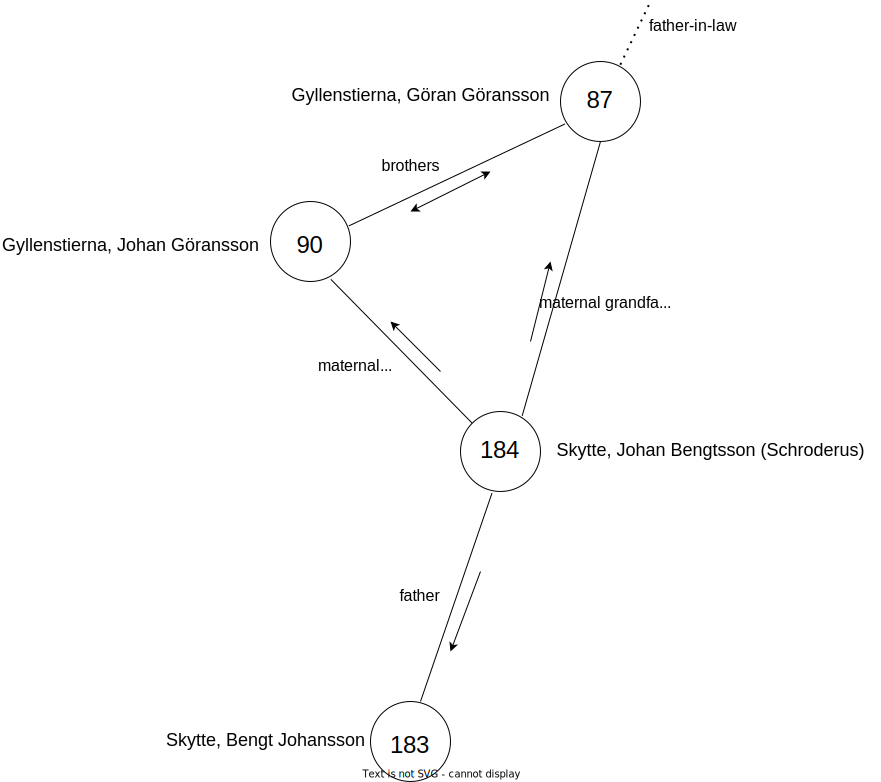
\includegraphics[scale=0.25]{example_network.drawio.png}
	\centering	
\end{figure}
In this context the graph's nodes depict individual councilors with the input of name and id number. Correspondingly the edges represent the kinships between two nodes. For instance, in Figure 1 we can see that Johan Bengtsson (Schroderus) Skytte (id 184) is Bengt Johansson Skytte's (id 183) father and a maternal grandfather for Johan Göransson Gyllenstierna (id 90) and Göran Göransson Gyllenstierna (id 87). Johan Göransson and Göran Göransson are brothers, however, their father is not mentioned in the dataset.\footfullcite{councilorsDS} 

\subsection{Implementation of the network analysis}


\end{document}
